\chapter{Introduction}
\label{chap:introduction}
\begin{figure}[t]
    \centering
    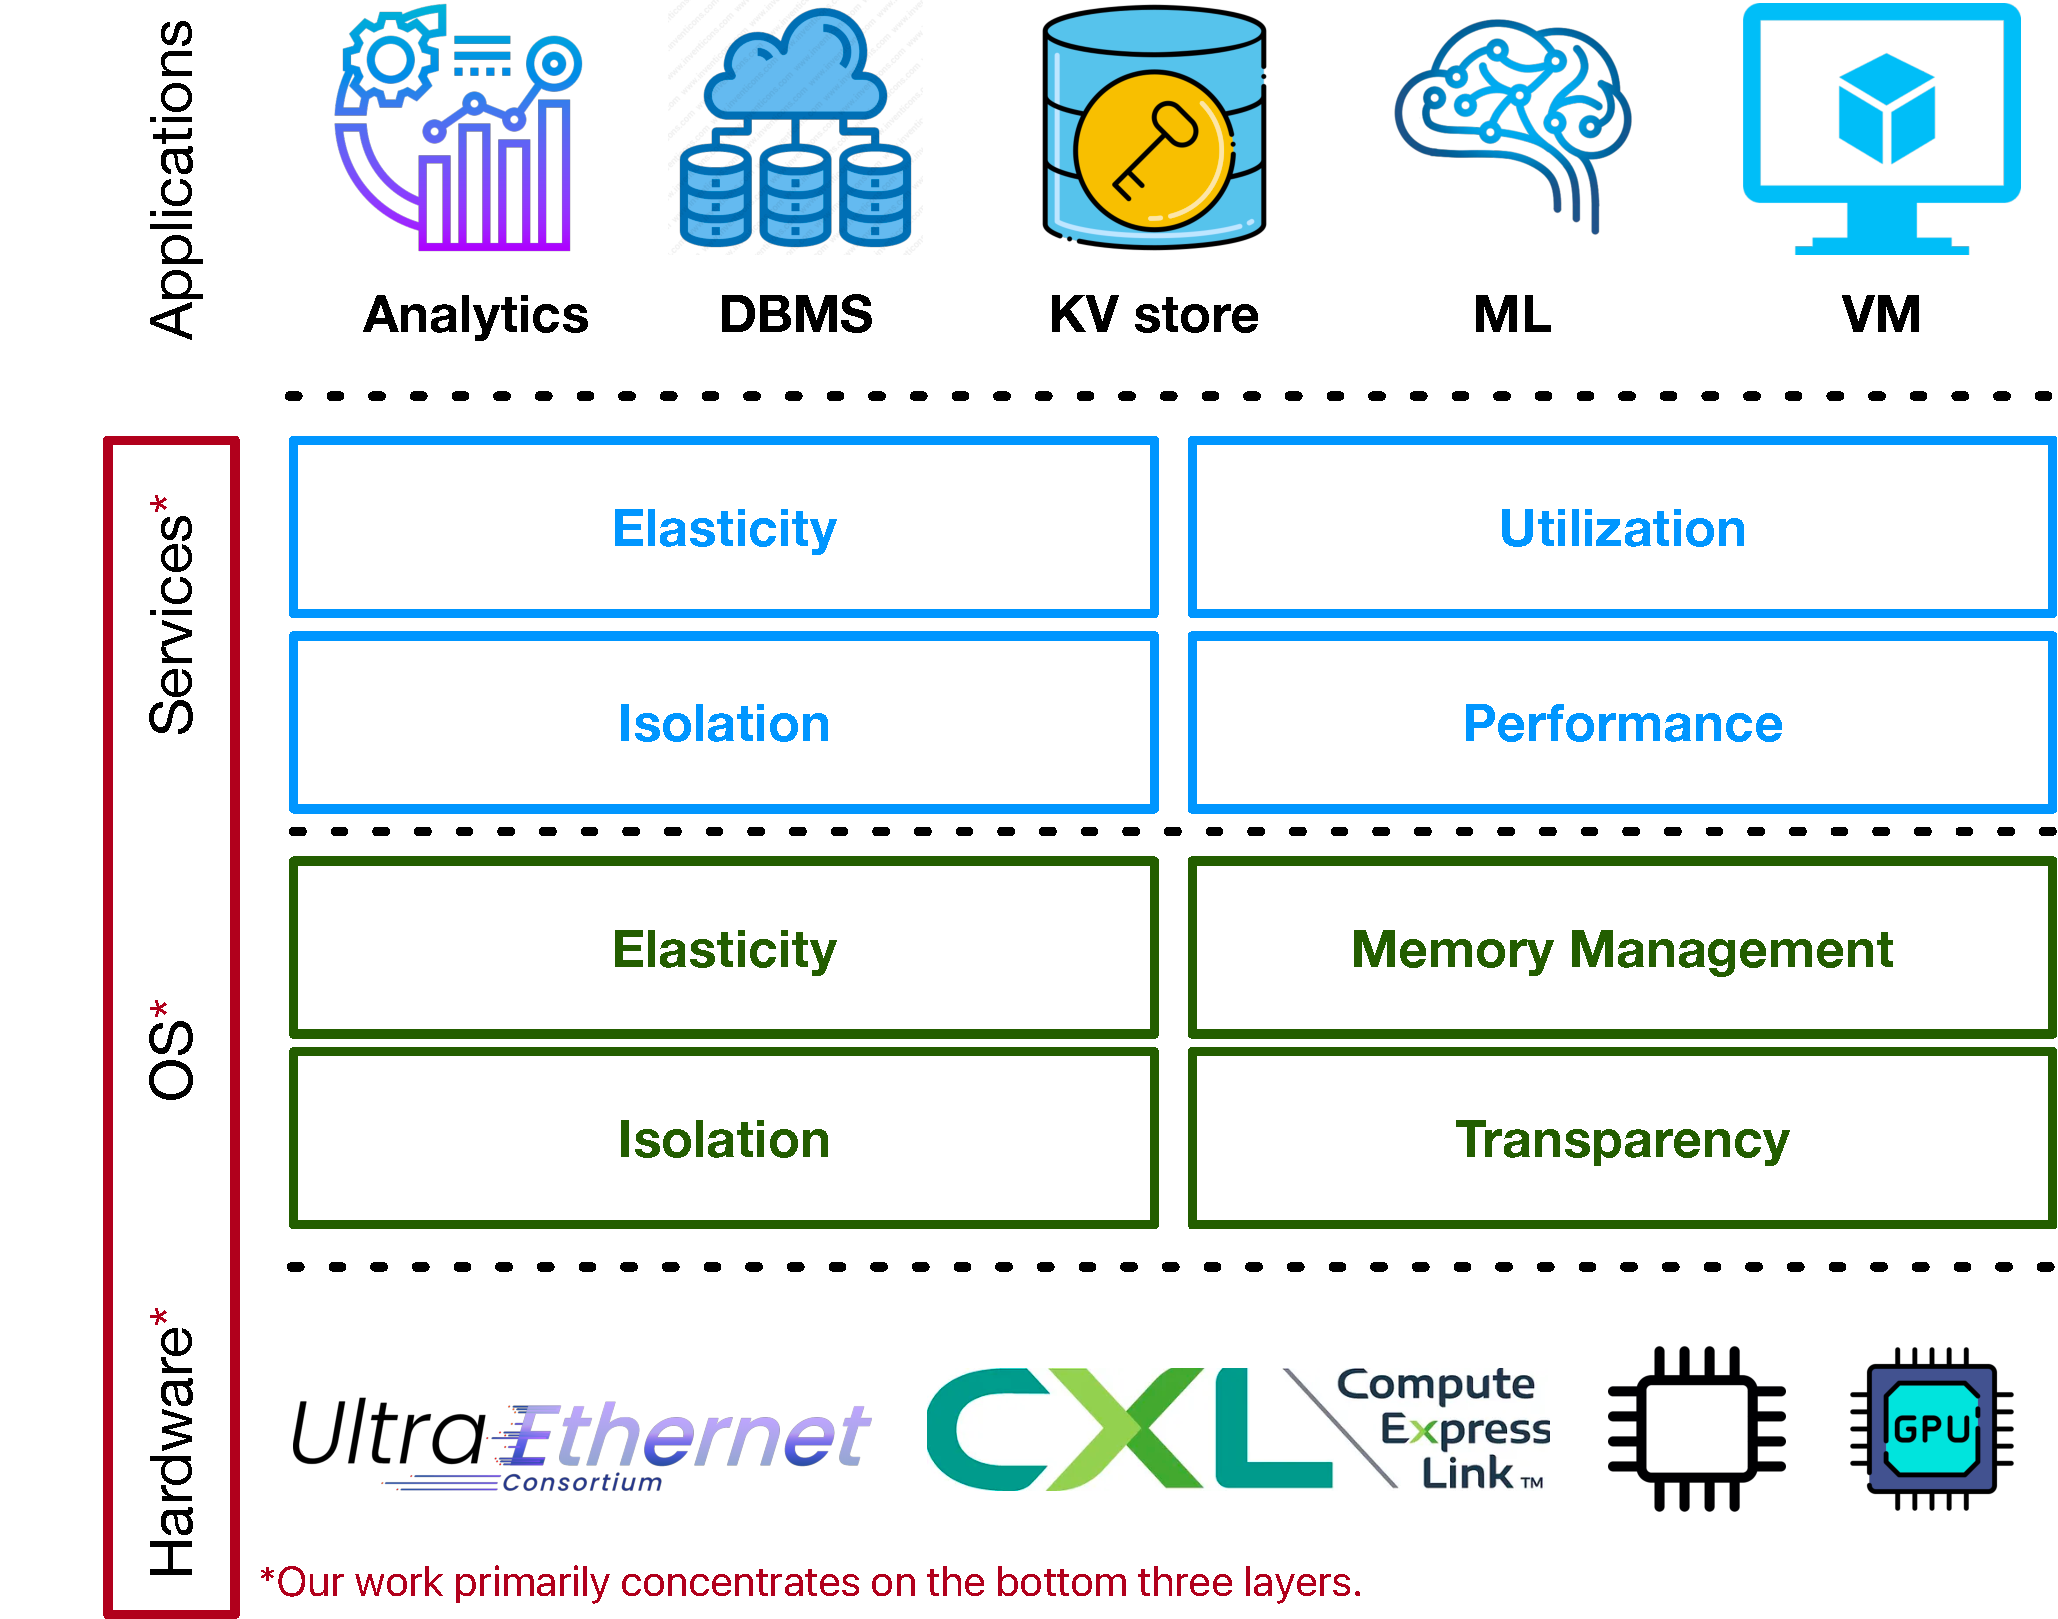
\includegraphics[width=0.7\columnwidth]{stack.pdf}
      \caption[Cloud Stack of Disaggregated Architecture]{\textbf{Cloud Stack of Disaggregated Architecture.} The service layer offers a specialized memory management interface tailored to specific application needs, as discussed in Chapter~\ref{chap:service}. In contrast, the OS layer provides a more generic interface, prioritizing transparency to ensure applications can run without modification and without requiring awareness of underlying hardware details.} 
      \label{fig:stack}
\end{figure}
The growing demand for scalable and efficient data center architectures has led to the emergence of resource disaggregation~\cite{mind, legoos, disagg, memdisagg1, memdisagg2, memdisagg3, memdisagg4, memdisagg5, memdisagg6}. This modern paradigm represents a significant shift from traditional monolithic server architectures. In conventional setups, servers are typically equipped with a fixed combination of compute, memory, and storage resources. In contrast, resource-disaggregated systems physically separate these resources and distribute them across various interconnects, such as networks~\cite{disagg, legoos, mind}, CXL~\cite{cxl, cxlasic}, and others. This separation allows for more flexible resource allocation and utilization.

Within the broader context of resource disaggregation in modern data center architectures, \textbf{memory disaggregation}~\cite{memdisagg1, memdisagg2, memdisagg3, memdisagg4, memdisagg5, memdisagg6} plays a crucial and foundational role. In traditional monolithic architecture, memory often becomes a bottleneck, limiting the scalability and adaptability of applications. This issue has been frequently observed and reported in production data centers~\cite{memory1, memory2, memory3, memory4, memory5, memory6, memory7, memory8, memory9, memory10}. By decoupling memory resources from compute and storage elements and presenting them as pooled, disaggregated resources~\cite{pool1, pool2}, data centers can achieve increased efficiency, scalability, and adaptability. Memory-intensive applications~\cite{redis, ramcloud, sparkmemory} can access the memory they need on demand, without being constrained by the limitations of individual servers. Memory disaggregation is the first step toward realizing the full potential of resource disaggregation, enabling data centers to efficiently allocate and utilize resources based on dynamic application needs. 


\section{Limitations of Existing Approaches}

While memory disaggregation offers several advantages, transitioning existing applications to this new architecture is far from straightforward. Recent research has proposed multiple approaches to address this challenge. Some efforts focus on optimizing applications for disaggregated memory~\cite{farm, aifm, sherman, existing1}, while others aim to transparently port existing applications, shifting the responsibility of performance mitigation to the service or operating system layer~\cite{mind, legoos, fastswap, infiniswap, runtime1, runtime2}. Additionally, hardware innovations complicate the matter further, as different interconnects, such as Ethernet and CXL, offer diverse interfaces and performance characteristics, complicating the standardization of software stack designs.


The fundamental challenge arises from the mismatch between the existing cloud stack, which was originally designed for monolithic architectures, and the demands of disaggregated architectures (Figure~\ref{fig:stack}). Current cloud and hardware stacks are not inherently designed to account for the unique characteristics of disaggregated memory, such as the physical decoupling of resources and the increased access latency due to interconnects. This misalignment introduces distinct challenges across various layers of the stack:


\paragraph{Application Interface} In disaggregated architectures, applications face unique challenges compared to traditional monolithic systems. The key difference stems from resource distribution: compute, memory, and storage are spread across multiple resource nodes instead of centralized in a single server. This distribution requires complex communication and data management strategies to account for increased latency and resource coordination. Moreover, transparency becomes a critical concern. There is an inherent trade-off between the benefits of resource disaggregation and the associated performance overhead. Application developers may need to either significantly redesign their applications for more efficient resource management or rely on cloud providers to integrate resource management at the service or operating system layer to facilitate smoother transitions.

\paragraph{Operating System Support} Unlike monolithic servers where the operating system (OS) manages resources within a single machine, the role and placement of the OS in disaggregated architectures remain topics of active debate in both academia and industry. Some approaches centralize OS functionality~\cite{mind, chase}, while others propose disaggregating the OS across resource nodes~\cite{legoos}, each offering its own advantages and challenges.

\paragraph{Performance Overheads} Transparently transitioning existing applications to a disaggregated architecture introduces several performance challenges. These include managing memory partitioning~\cite{jiffy} and dealing with applications exhibiting irregular memory access patterns~\cite{chase}. Other factors, such as latency sensitivity, bandwidth limitations, and the overhead of managing remote resources, exacerbate the performance penalties that must be carefully mitigated in disaggregated systems.

\paragraphb{Future Interconnects} The use of networks as interconnects for resource disaggregation has been a focus of research in both academia and industry. However, networks face inherent challenges, such as performance slowdowns compared to intra-server resource access and the absence of built-in coherency. Emerging hardware technologies like Compute Express Link (CXL)~\cite{cxl, cxlasic, pond} offer promising improvements, including faster access times and hardware-supported cache coherence. Despite this potential, current hardware prototypes and software support for these technologies are still in early stages, and their full impact on software design remains uncertain.

\section{Thesis Overview}

In this dissertation, we attempt to take a top-down approach and explore the optimal memory management solutions for three most significant layers, i.e. Service, OS and Hardware layers of disaggregated memory architectures.

\subsection{Service Layer: Memory Management as a Service}
At the layer closest to the application, we explore the design requirements and challenges of providing memory management as a service. This service manages a pool of memory resources and makes them available to applications. We propose an end-to-end system design, \textit{Jiffy}, which enables multiple applications to efficiently share memory resources in an elastic manner. Jiffy also provides interfaces for common data structures, making it applicable to a wide range of cloud applications.

\subsection{OS Layer: In-Network Memory Management}

While applications may rely on Jiffy for managing memory resources, we take a deeper approach by focusing on the Operating System (OS) as the manager of disaggregated memory. This approach allows applications to run transparently, benefiting from the decoupled architecture without requiring significant modification. In disaggregated systems, there is no single host to manage resources, a task traditionally handled by the OS. We propose a novel OS design that integrates resource management into the network interconnect itself. Starting with a system called \textit{MIND}, we tackle critical challenges such as memory address translation, memory protection, and cache coherence across multiple nodes. Although this design performs well for cache-friendly workloads, it struggles with cache-unfriendly applications due to the overhead of interconnect communication. To address this, we introduce \textit{PULSE}, a near-memory accelerator designed specifically for pointer traversal workloads. PULSE provides a simple, effective interface that can be seamlessly integrated into existing cloud applications.

\subsection{Hardware Layer: Memory Management for Next-Gen Interconnects}
Previous work~\cite{mind, legoos} has largely relied on Ethernet as the primary interconnect for disaggregated data centers. However, with the rise of new memory interconnects such as CXL, memory management must adapt to these emerging technologies. New challenges arise, particularly in managing multiple tiers of memory efficiently across applications. We begin by evaluating the performance of CXL 1.1 extended memory in a single-host environment and then explore how modern data center applications can benefit from such disaggregated memory systems.

\section{Outline and Previously Published Work}

This dissertation is organized as follows. Chapter~\ref{chap:service} introduces Jiffy, a distributed memory management system that decouples memory capacity and lifetime from compute in the serverless paradigm. Chapter~\ref{chap:os} describes two innovated system design: (1) MIND, a rack-scale memory disaggregation system that uses programmable switches to embed memory management logic in
the network fabric. (2) PULSE, a framework centered on enhancing in-network optimizations for
irregular memory accesses within disaggregated data centers. Chapter ~\ref{chap:hardware} presents our exploration in latest Compute Express Link(CXL) hardware. We conclude with our contributions and possible future work directions in Chapter~\ref{chap:future}.

Chapter~\ref{chap:service} revises material from~\cite{jiffy}\footnote{Work done in collaboration with Rachit Agarwal, Aditya Akella, and Ion Stoica}. Chapter~\ref{chap:os} revises material from~\cite{mind}\footnote{Work done in collaboration with Seung-seob Lee, Yanpeng Yu, Lin Zhong and Abhishek Bhattacharjee} and~\cite{chase}\footnote{Work done in collaboration with Seung-seob Lee and Abhishek Bhattacharjee}. Finally, Chapter~\ref{chap:hardware} revises material from~\cite{cxleurosys}\footnote{Work done in collaboration with the Bytedance Infrastructure team}.
